% arara: clean: {
% arara: --> extensions:
% arara: --> ['log','idx','ilg','ind','out','bbl','blg','thm','toc','aux','synctex.gz','bcf','run.xml','contb',
% arara: --> 'contg','contn','diffb','diffg','diffn','funb','fung','funn','genb','geng','genn','intb','intg','pytxcode',
% arara: --> 'intn','limb','limg','limn','logb','logg','logn','realb','realg','realn','seqb','seqg','seqn','ist',
% arara: --> 'serb','serg','sern','setb','setg','setn','ssfunb','ssfung','ssfunn','topb','topg','topn','pdf']
% arara: --> }
% arara: pdflatex
% arara: pdflatex
% arara: clean: {
% arara: --> extensions:
% arara: --> ['log','idx','ilg','ind','out','bbl','blg','thm','toc','aux','synctex.gz','bcf','run.xml','contb',
% arara: --> 'contg','contn','diffb','diffg','diffn','funb','fung','funn','genb','geng','genn','intb','intg','pytxcode',
% arara: --> 'intn','limb','limg','limn','logb','logg','logn','realb','realg','realn','seqb','seqg','seqn','ist',
% arara: --> 'serb','serg','sern','setb','setg','setn','ssfunb','ssfung','ssfunn','topb','topg','topn']
% arara: --> }
\PassOptionsToPackage{svgnames}{xcolor}
\documentclass[spanish,10pt,utf8,handout]{beamer} %
\usepackage[T1]{fontenc}
\usepackage{mathpazo}
\usepackage[spanish]{babel}
\usepackage{amsmath,mathrsfs,amsfonts,amsthm}
\usepackage{enumitem}

\usepackage[backend=biber,style=numeric, defernumbers=true, sorting=ynt,maxbibnames=4,maxcitenames=4]{biblatex}
\addbibresource{bibliography/reference.bib}
% https://tex.stackexchange.com/questions/410249/conflict-between-marvosym-and-mathabx
\newcommand{\MVAt}{{\usefont{U}{mvs}{m}{n}\symbol{`@}}}
\renewcommand{\spanishfigurename}{Figura}
\renewcommand{\spanishcontentsname}{Índice analítico}
\renewcommand{\listingscaption}{Programa}

% https://tex.stackexchange.com/questions/68080/beamer-bibliography-icon
\setbeamertemplate{bibliography item}{%
	\ifboolexpr{ test {\ifentrytype{book}} or test {\ifentrytype{mvbook}}
		or test {\ifentrytype{collection}} or test {\ifentrytype{mvcollection}}
		or test {\ifentrytype{reference}} or test {\ifentrytype{mvreference}} }
	{\setbeamertemplate{bibliography item}[book]}
	{\ifentrytype{online}
		{\setbeamertemplate{bibliography item}[online]}
		{\setbeamertemplate{bibliography item}[article]}}%
	\usebeamertemplate{bibliography item}}

\defbibenvironment{bibliography}
{\list{}
	{\settowidth{\labelwidth}{\usebeamertemplate{bibliography item}}%
		\setlength{\leftmargin}{\labelwidth}%
		\setlength{\labelsep}{\biblabelsep}%
		\addtolength{\leftmargin}{\labelsep}%
		\setlength{\itemsep}{\bibitemsep}%
		\setlength{\parsep}{\bibparsep}}}
{\endlist}
{\item}
%\usetheme[numbering=fullbar]{focus}%progressbar
%\definecolor{main}{RGB}{92, 138, 168}
%\definecolor{background}{RGB}{240, 247, 255}
\usepackage[
	audience=english
%	audience=spanish,
%	audience=german
]{beameraudience}

%\newcommand{\progressbar}{%
%	\pgfmathsetmacro{\theta}{360/\inserttotalframenumber*\insertframenumber}
%	\begin{tikzpicture}[scale=0.035]
%	\fill[yellow] (0,0) circle (9);
%	\fill[red] (0,0) -- (9,0) arc (0:-\theta:9);
%	\fill[white] (0,0) circle (5);
%	\node at (0,0) {\insertframenumber};
%	\end{tikzpicture}
%}

%\setbeamertemplate{footline}{\hfill \progressbar}
\usepackage{textpos}
\usepackage{mathtools}
\usepackage{dsfont}
%\useoutertheme{splitwithminiframes}
%\useoutertheme{sidebarwithminiframes}
%\usecolortheme[cautious]{owl}
\theoremstyle{definition}
\newtheorem{remark}{Observación}

\usetheme{CambridgeUS}
\usecolortheme{dolphin}
\useinnertheme{rectangles}
%\useoutertheme[hooks]{tree}

\usefonttheme[onlymath]{serif}

%\setbeamercovered{transparent}
\setbeamercovered{dynamic}

\setbeamertemplate{background canvas}{
\includegraphics[height=\paperheight]{background}}
\setbeamertemplate{footline}[frame number]{}
\setbeamertemplate{navigation symbols}{}
\setbeamertemplate{footline}{}
\setbeamertemplate{headline}{}
\setbeamertemplate{blocks}[rounded][shadow=false] 

\addtobeamertemplate{block begin}{\pgfsetfillopacity{0.6}}{\pgfsetfillopacity{1}}
\addtobeamertemplate{block alerted begin}{\pgfsetfillopacity{0.6}}{\pgfsetfillopacity{1}}
\addtobeamertemplate{block example begin}{\pgfsetfillopacity{0.6}}{\pgfsetfillopacity{1}}

\title[Teorema de los cuatro colores]{\Huge\sffamily Relaciones de recurrencias}
\subtitle{Ecuaciones en diferencias y análisis en escalas de tiempo}

\author[Grupo N$^\circ6$]{%
	\texorpdfstring{%
		\begin{columns}
			\column{.3\linewidth}
			\centering
			C. Aznarán Laos %\inst{1,2}
			\column{.3\linewidth}
			\centering
			F. Cruz Ordoñez %\inst{1,2}
		\end{columns}
		\vspace{12pt}
		\begin{columns}
			\column{.3\linewidth}
			\centering
			G. Quiroz Gómez %\inst{1,2}
			\column{.3\linewidth}
			\centering
			J. Micha Velasque %\inst{1,2}
		\end{columns}
		\vspace{12pt}
		\begin{columns}
			\column{.3\linewidth}
			\centering
			D. García Fernández %\inst{1,2}
%			\column{.3\linewidth}
			\centering
		\end{columns}
	}
	{Author 1, Author 2, Author 3}
}

\institute[FC -- UNI]{\large%\inst{1}
	Facultad de Ciencias \and%\inst{2}
	Universidad Nacional de Ingeniería
}
\date{25, 27 de junio del 2019}

\graphicspath{{images/}}

\AtBeginSubsection[]
{
	\begin{frame}<beamer>
		\frametitle{\contentsname}
		\tableofcontents[
		currentsection,
		sectionstyle=show/show,
		subsectionstyle=show/shaded/hide%-show/shaded/hide
		]
	\end{frame}
}
%\includeonlyframes{%
%	toc,%
%}
\begin{document}

\frame{\titlepage} %\begin{frame}[plain]\maketitle\end{frame}
\begin{frame}[label=toc]{\contentsname}\transblindsvertical
	\tableofcontents
\end{frame}
\section{Introducción}
\subsection{Relación de recurrencia}

\subsubsection{Con coeficientes constantes}

\subsubsection{Homogénea}
\section{Ecuación en diferencias}\label{sec:difference}\index{Ecuación en diferencias!definición}

Aquí es conveniente representar cualquier sucesión de números reales $(a_{n})_{n} $ como la función $f\colon\mathds{N}\rightarrow\mathds{R}$ definido por: \[ f(n)=a_{n},\quad\forall n\in\mathds{N}. \] Dadas dos funciones $f,g\colon\mathds{N}\rightarrow\mathds{R}$ y $r\in\mathds{R} $ consideremos las funciones: \[ (f+g)(n)=f(n)+g(n),\quad\text{y}\quad(rf)(n)=rf(n)\quad\forall n\in\mathds{N}. \] Dotado de estas operaciones, el conjunto de funciones de $\mathds{N}\rightarrow\mathds{R}$ es un $\mathds{R}$--espacio vectorial de funciones. También consideraremos la función: \[ (fg)(n)=f(n)g(n)\forall k\in\mathbb{N}. \] Un mapa lineal del espacio de funciones de $\mathds{N}$ a $ \mathds{R}$ en sí mismo es un operador.

\begin{definition}[Operador identidad y operador de cambio]
Consideramos el espacio de funciones de $\mathds{N}\to\mathds{R}$. Para cada función $f\colon\mathds{N}\rightarrow\mathds{R}$ el operador identidad y el operador de cambio $\theta$ están definidos: \[ \mathds{I}(f)=f\quad\text{y}\quad\theta(f)(n)=f(n+1)\quad\forall n\in\mathds{N}. \] Uno verifica inmediatamente que la identidad y el operador de cambio son de hecho lineales.
\end{definition}

\begin{proposition}[Linealidad de la identidad y el operador de cambio]
Sean las funciones $f,g\colon\mathds{N}\to\mathds{N}$ y $c\in\mathds{R}$. Luego tenemos:
\begin{enumerate}
	\item $\mathds{I}\left(f+g\right)(n)=\mathds{I}(f)(n)+\mathds{I}(g)(n)$.
	\item $\mathds{I}\left(cf\right)(n)=c\mathds{I}(f)(n)$ y $\theta\left(cf\right)(n)=c\theta(f)(n)$.
\end{enumerate}
\end{proposition}

\begin{proof}
	Sea $n\in\mathds{N}$, luego:
	\begin{align*}
	\theta(f+g)(n)&=(f+g)(n+1)=f(n+1)+g(n+1)=\theta(f)(n)+\theta(g)(n).\\
	\theta(cf)(n)&=(cf)(n+1)=cf(n+1)=c\theta(f)(n).
	\end{align*}
	Se verifica la linealidad de $\mathds{I}$ inmediatamente.
\end{proof}

Para cualquier operador $T$, será conveniente un ligero abuso de notación, para escribir $Tf(n)$ en lugar de $T(f)(n)$. Además en algunos casos, por ejemplo cuando $f$ depende de otros parámetros, uno escribe $T_{n}f(n)$ en lugar de $Tf(n)$ para evitar la ambigüedad. Así, por ejemplo, denotada por $\mathds{I}_{\mathds{N}}\colon\mathds{N}\rightarrow\mathds{N}$ la función definida por $\mathds{I}_{\mathds{N}}(n)=n$ para cada $n\in\mathds{N} $ escribiremos $\theta n=n+1$ en lugar de $\theta(\mathds{I}_{\mathds{N}})(n)=n+1$. Análogamente $\theta n^{2}=(n+1)^{2}$, $\theta_{n}n^{a}=(n+1)^{a}$ y $\theta_{n}a^{n}=a^{n+1}$ para cada $a\in\mathds{R}$.

Para las funciones de valor real de una variable de número natural ahora introducimos el análogo de la derivada habitual para funciones de valor real de una variable real:

\begin{definition}[Operador de cambio]
	El operador diferencia es el operador $\bigtriangleup$ que a cada función $f\colon\mathds{N}\rightarrow\mathds{R}$ asigna la función $\bigtriangleup f\colon\mathds{N}\rightarrow \mathds{R}$, definido de la siguiente manera: \[ \bigtriangleup f(n)=f(n+1)-f(n),\quad\forall n\in\mathds{N}. \]
\end{definition}

\begin{remark}
	Usando el operador de cambio, uno tiene $\bigtriangleup=\theta-\mathds{I}$, es decir: \[ \bigtriangleup f=\theta f-f,\quad\forall f\colon\mathds{N}\rightarrow\mathds{R}. \] Claramente, para cada función $f\colon\mathds{N}\rightarrow\mathds{R}$, uno tiene: \[ \bigtriangleup f(k)=\frac{f(k+1)-f(k)}{1}, \] entonces $\bigtriangleup f\colon\mathds{N}\rightarrow\mathds{R}$ es una función que mide el cociente de diferencia de $f$ sobre el intervalo más pequeño posible de números naturales, es decir, un intervalo de longitud uno. En este sentido, el operador diferencia constituye el análogo discreto de la noción de derivada para funciones de una variable real. En lo que sigue, el lector tendrá ocasión para anotar analogías y contrastes entre estas dos nociones.
\end{remark}

Al igual que la derivada, el operador de diferencia es lineal: de hecho, es una diferencia de dos operadores lineales.

\begin{proposition}[Linealidad de la diferencia]
	Sean $ f,g\colon\mathds{N}\rightarrow\mathds{R}$ y $c\in\mathds{R}$. Luego uno tiene:
	\begin{enumerate}
		\item $\bigtriangleup\left(f+g\right)=\bigtriangleup f+\bigtriangleup g$.
		\item $\bigtriangleup(cf)=c\bigtriangleup f$.
	\end{enumerate}
\end{proposition}


\begin{proof}
	Como $ \bigtriangleup=\theta-\mathds{I}$ se obtiene:
	\begin{enumerate}
		\item $\bigtriangleup\left(f+g\right)=\left(\theta-\mathds{I}\right)\left(f+g\right)=\theta\left(f+g\right)-\mathds{I}\left(f+g\right)=\theta(f)-f+\theta(g)-g=\bigtriangleup(f)-\bigtriangleup(g)$.
		\item $\bigtriangleup\left(cf\right)=\left(\theta-\mathds{I}\right)\left(cf\right)=\theta\left(cf\right)-\mathds{I}\left(cf\right)=c\theta(f)-cf=c(\theta-\mathds{I})(f)=c\bigtriangleup(f)$.
	\end{enumerate}
\end{proof}
Ahora vemos cómo el operador de diferencia actúa en algunas funciones simples con dominio $\mathds{N}$.

\begin{example}\leavevmode
	\begin{enumerate}
		\item Funciones constantes: al igual que en el caso de la derivada de una  constante. Funciona con dominios en $\mathds{R}$, aquí también tenemos que la diferencia de una función constante (con dominio $\mathds{N}$) es igual a la función cero: de hecho, si $f(n)=c\in\mathds{R}$ por cada $n\in\mathds{N}$, entonces \[ \bigtriangleup f(k)=f(k+1)-f(k)=c-c=0. \]
		\item Función de identidad en los números naturales: al igual que en el caso continuo, la diferencia de la función de identidad $I_{\mathds{N}}\colon\mathds{N}\rightarrow \mathds{N}$ es la función constante $n=1$ para todo $n\in\mathds{N}$. De hecho, \[ \bigtriangleup I_{\mathds{N}}(n)=I_{\mathds{N}}(n+1)-1=n+1-n=1. \]
		\end{enumerate}
\end{example}

\begin{example}
	Los operadores de cambio y diferencia conmutan. Más explícitamente, uno tiene \[ \bigtriangleup\circ\theta=\theta\circ\bigtriangleup. \]
\end{example}

\begin{proof}
De hecho, para cada $n\in\mathds{N} $ y cada función $f\colon\mathds{N}\rightarrow\mathds{R}$ uno tiene
	\begin{align*}
		\bigtriangleup\left(\theta f\right)(n)&=\theta f\left(n+1\right)-\theta f(n)=f(n+2)-f\left(n+1\right),\\
		\shortintertext{mientras}
		\theta\left(\bigtriangleup f\right)(n)&=\bigtriangleup f\left(n+1\right)=f(n+2)-f(n+1).
	\end{align*}
Por lo tanto, uno tiene $\bigtriangleup\left(\theta f\right)=\theta\left(\bigtriangleup f\right)(n)$.
\end{proof}
La fórmula para la diferencia de un producto se parece a la del derivado de un producto, excepto la introducción del operador de turno:
\begin{proposition}[Diferencia de un producto]
Si $f,g\colon\mathds{N}\rightarrow\mathds{R}$, luego \[ \bigtriangleup\left(fg\right)=\bigtriangleup f\theta g+f\bigtriangleup g. \]
\end{proposition}

\begin{remark}
	Cabe destacar el hecho evidente de que a pesar de la aparente falta de simetría, uno tiene $\bigtriangleup\left(fg\right)=\bigtriangleup\left(gf\right)$.
\end{remark}

\begin{proof}
	\begin{align*}
		\bigtriangleup\left(f(n)g(n)\right)
		&=f\left(n+1\right)g\left(n+1\right)-f(n)g(n)\\
		&=f(n+1)g(n+1)-f(n)g(n+1)+f(n)(n+1)-f(n)g(n)\\
		&=(f(n+1)-f(n))g(n+1)+f(n)g(n+1)-g(n)\\
		&=\bigtriangleup f(n)\theta g(n)+f(n)\bigtriangleup g(n).
	\end{align*}
\end{proof}

\

Una ecuación en diferencias es una expresión de la forma: \[ G\left(n,f(n),f(n+1),\ldots,f(n+k)\right)=0,\forall n\in\mathds{Z} \] donde $f$ es una función definida en $\mathds{Z}$.

Si después de simplificar esta expresión quedan los términos $f\left(n+k_{1}\right)$ y $f\left(n+k_{2}\right)$ como el mayor y el menor, respectivamente. Se dice que la ecuación es de orden $k=k_{1}-k_{2}$.

\begin{example}[Ecuación en diferencias de orden $3$]
	La ecuación dada por \[ 5f(n+4)-4f(n+2)+f(n+1)+(n-2)^{3}=0 \] es de orden $4-1=3$.
\end{example}

Una ecuación en diferencias de orden $k$ se dice que es \emph{lineal}\index{Ecuación en diferencias!lineal} si puede expresarse de la forma: \[ p_{0}(n)f(n+k)+p_{1}(n)f(0+k-1)+\cdots+p_{k}(n)f(n)=g(n), \] donde los coeficientes $p_{i}$ son funciones definidas en $\mathds{Z}$.

El caso más sencillo es cuando los coeficientes son constantes $p_{i}(n)=a_{i}$: \[ a_{0}f(n+k)+a_{1}f(n+k-1)+\cdots+a_{k}f(n)=g(n). \] La ecuación en diferencias se dice que es \emph{homogénea}\index{Ecuación en diferencias!homogénea} en el caso que $g(n)=0$, y completa en el caso contrario.

\begin{theorem}{}
	Dada la ecuación en diferencias lineal de coeficientes constantes y de orden $ K $: \[ a_{0}f(n+k)+a_{1}f(n+k-1)+\cdots+a_{k}f(n)=g(n) \] el problema de hallar una función definida $\mathds{Z}$, que verifique la ecuación, y tales que en los $k$ enteros consecutivos $n_{0},n_{0}+1,\ldots,n_{0}+k-1$ tome los valores dados $c_{0},c_{1},\ldots,c_{k-1}$, tiene solución única.
\end{theorem}

\begin{theorem}{}
	Dada una ecuación en diferencias lineal homogénea de coeficientes constantes y de orden $k$. Si una solución $f$ es nula en $k$ enteros consecutivos, entonces $f$ es idénticamente nula.
\end{theorem}

\begin{theorem}{}
	Toda combinación lineal de soluciones de una ecuación en diferencias lineal homogénea de coeficientes constantes y de orden $k$ es también solución de dicha ecuación.
\end{theorem}

\begin{definition}[Solución de una ecuación en diferencias homogénea]
Sea la ecuación en diferencias lineal homogénea de coeficientes constantes y de orden $k$. \[ a_{0}f(n+k)+a_{1}f(n+k-1)+\cdots+a_{k}f(n)=0,\quad\forall k\in\mathds{Z}. \] Buscaremos soluciones del tipo $f(n)=r^{n}.$ Entonces, \[ r^{n}\left(a_{0}r^{k}+a_{1}r^{k-1}+\cdots+a_{k}\right)=0\implies r^{n}(a_{0}r^{k}+a_{1}r^{k-1}+\cdots+a_{k})=0. \] Por tanto, $r$ es raíz de la \textbf{ecuación característica} \[ (a_{0}r^{k}+a_{1}r^{k-1}+\cdots+a_{k})=0. \]
\end{definition}

El estudio de la solución dependería de si las raíces de la ecuación característica son simples o múltiples.
\begin{example}
	Hallar la solución de \[ f(n+2)-4f(n+1)+3f(n)=0\quad\forall n\in\mathds{Z},\quad f(0)=0,\quad f(1)=1. \] La ecuación característica es \[ r^{2}-4r+3=0\rightarrow r_{1}=3,\quad r_{2}=1. \] Por lo tanto: \[ f(n)=c_{1}3^{n}+c_{2}1^{n}=c_{1}3^{n}+c_{2}. \] Por otra parte:
	\begin{equation*}
	\left.\begin{aligned}
	f(0)&=\phantom{1}c_{1}+c_{2}=0\\
	f(1)&=3c_{1}+c_{2}=1
	\end{aligned}
	\right\}
	\longrightarrow c_{1}=\frac{1}{2},\quad c_{2}=-\frac{1}{2}.
	\end{equation*}
De donde \[ f(n)=\frac{1}{2}\cdot3^{n}-\frac{1}{2}=\frac{3^{n}-1}{2}. \]
\end{example}
\section{Ecuaciones de recurrencia}

\begin{frame}
\frametitle{\secname}

\textit{Resolver una ecuación de recurrencia} significa encontrar una sucesión que satisfaga las ecuaciones de recurrencia.

\

Encontrar una ``solución general'' significa encontrar una fórmula que describe todas las soluciones posibles (todas las sucesiones posibles que satisfacen la ecuación).

\

Veamos el siguiente ejemplo:

\begin{claim}
	Considere que $T_{n}$ satisface la siguiente ecuación
	\begin{equation}
	T_{n}=2T_{n-1}+1\quad\forall n\in\mathds{N}\setminus\left\{1\right\}.
	\end{equation}
\end{claim}

\end{frame}

\subsection{Ejemplos definidos por ecuaciones de recurrencia}

\begin{frame}
\frametitle{\subsecname}

\begin{example}[Desajustes]
	Imagine una fiesta donde las parejas llegan juntas, pero al final de la noche, cada persona se va con una nueva pareja. Para cada $n\in\mathds{N}$, digamos que $D_{n}$ es el número de diferentes formas en que las parejas pueden ser ``trastornadas'', es decir, reorganizadas en parejas, por lo que ni uno está emparejado con la persona con la que llegaron.
\end{example}

\begin{claim}[$D_{n}$ para cualquier valor de $n$]
	Para todo $n\geq4$ tendremos: \[ D_{n}=(n-1)\left\{D_{n-2}+D_{n-1}\right\}. \] Y la sucesión definida en $\mathds{N}$ es \[ S_{n} = A \times n!. \]
\end{claim}

\end{frame}

\begin{frame}
\frametitle{\subsecname}

\begin{theorem}[Desigualdad para la acotación de $D_{n}$]
Para todo $n\geq2$ tenemos: \[ \left(\frac{1}{3}\right)n!\leq D_{n}\leq\left(\frac{1}{2}\right)n!. \]
\end{theorem}

La mejor fórmula para $D_{n}$ que sabemos utiliza la función de ``entero más cercano''.

\begin{definition}
	Para cualquier número real $x$, se define \textbf{el entero más cercano a} $x$, $\lceil x\rfloor$:

	Si $x$ es escrito como $n+f$ donde $n$ es el entero $\lfloor x\rfloor$, y $f$ es una fracción donde $0\leq f<1$:

	\begin{itemize}
		\item Si $0\leq f<\frac{1}{2}$, entonces $\lceil x\rfloor=n$.
		\item Si $\frac{1}{2}\leq f<1$, entonces $\lceil x\rfloor=n+1$.
	\end{itemize}
\end{definition}

\begin{remark}
	Entonces $D_{n}=\lceil(n!)/e\rfloor$ cuando $e=2.71828182844\ldots$ es la base del logaritmo natural.

	$(n!)/e$  nunca es igual a $\lceil(n!)/e\rfloor+\frac{1}{2}$.
\end{remark}
\end{frame}

\subsubsection{Función de Ackermann}

\begin{frame}
\frametitle{\subsubsecname}
A finales de 1920's, el lógico y matemático alemán, discípulo de David Hilbert, Wilhelm Ackermann (1896–1962), dio un ejemplo de una función computable total que no es recursiva primitiva.

\begin{minipage}{0.45\paperwidth}
	\begin{definition}[Ackermann]
		Sea $A\colon\mathds{N}\times\mathds{N}\rightarrow\mathds{N}$ una función. Se define recursivamente usando tres reglas:
		\begin{enumerate}
			\item $A(1,n)=2$, $\forall n\geq 1$.
			\item $A(m,1)=2m$, $\forall m\geq 2$.
			\item Cuando $m>1$ y $n>1$ se tiene: $A\left(m,n\right)=A\left(A(m-1,n),n-1\right)$.
		\end{enumerate}
	\end{definition}
	\begin{remark}
		Entonces $A\left(2,n\right)=4,\quad\forall n\geq1$. Además $A\left(m,2\right)=2^{m},\quad\forall m\geq 1$. Seguidamente se puede continuar a calcular $A\left(m,3\right)=2\uparrow m$ con la función torre definida por $2\uparrow\left[k+1\right]=2^{2\uparrow k}$ con valor inicial $2\uparrow 1=2$, por el P.I.M.
	\end{remark}
\end{minipage}
\hfill
\begin{minipage}{0.45\paperwidth}
	\begin{listing}[H]
		\inputminted{python}{./code/ackermann.py}
		\caption{Programa \texttt{ackermann.py}}
	\end{listing}
\end{minipage}

\end{frame}
\begin{frame}
	Hola
	\frametitle{Soluciones}
	%------------------------------------------------------------ 1
	\only<1>{
		\framesubtitle{The first frame subtitle}
		\begin{itemize}
			\item some text on slide 1
	\end{itemize}}
	%------------------------------------------------------------ 2
	\only<2>{
		\framesubtitle{The second frame subtitle}
		\begin{itemize}
			\item some text on slide 2
	\end{itemize}}
\end{frame}
\section{Realización numérica}
\subsection{Discretización}
\subsubsection{Método de Euler}
\subsubsection{Método de Runge-Kutta}
\subsection{Escalas de tiempo}
\subsubsection{Derivada fraccionaria}
\subsection{Módulo \texttt{timescale}}

\frame[t]{
	Una escala de tiempo es un conjunto cerrado $\mathds{T}$ bajo la topología estándar sobre $\mathds{R}$.

	Se define el operador salto posterior $\sigma\colon\mathds{t}\rightarrow\mathds{T}$ por \[ \sigma\left(T\right)\coloneqq\inf\left\{z\in\mathds{T}:z>t\right\} \]

	la granicidad $\mu\colon\mathds{T}\rightarrow\mathds{R}$ por \[ \mu\left(t\right)=\sigma\left(t\right)-t \] y función granicidad minimal $\mu_{\ast}\colon\mathds{T}\rightarrow\mathds{R}$ por \[ \mu_{\ast}\left(s\right)=\inf_{\tau\in\left[s,\infty\right)\cap\mathds{T}}\mu\left(t\right). \]

	Una función $f\colon\mathds{T}\rightarrow\mathds{C}$ es llamada $\Delta$--diferenciable si para cualquier $\varepsilon>0$ existe $\delta>0$ tal que para todo $s\in\left(t-\delta,t+\delta\right)\cap\mathds{T}$ y existe un número $f^{\Delta}\left(t\right)$ tal que \[ |\left[f\left(\sigma\left(s\right)\right)-f\left(s\right)\right]f^{\Delta}\left(s\right)\left[\sigma\left(t\right)-s\right]|\leq\varepsilon|\sigma\left(t\right)-s|. \]

	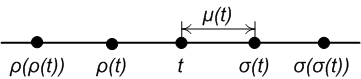
\includegraphics[width=0.4\paperwidth]{operators}
}

\frame{
	La integración se define de modo que $\int_{t}^{s}f^{\Delta}\left(\tau\right)\Delta\tau=f\left(t\right)-f\left(s\right)$.

	Si $\mathds{T}$ consiste únicamente de puntos aislados, entonces \[ f^{\Delta}\left(t\right)=\frac{f\left(\sigma\left(t\right)\right)-f\left(t\right)}{\mu\left(t\right)} \]

	y

\[
\int_{a}^{b}f\left(t\right)\Delta t=
\begin{cases}
	\sum_{t\in\left[a,b\right)\cap\mathds{T}}\mu\left(t\right)f\left(t\right),&\text{si }a<b.\\
	0, & \text{si } a = b.\\
	-\sum_{t\in\left[b,a\right)\cap\mathds{T}}\mu\left(t\right)f\left(t\right), & \text{si }a>b.
	\end{cases}
\]
}

%\includeslide{}
%\appendix
%\frame[noframenumbering,plain]{text}

\setbeamertemplate{footline}
{%
	\hbox{%
		\begin{beamercolorbox}[wd=.3\paperwidth,ht=7.8pt,dp=3pt,center]{author in head/foot}\insertshortauthor
		\end{beamercolorbox}%
		\begin{beamercolorbox}[wd=.4\paperwidth,ht=7.8pt,dp=3pt,center]{title in head/foot}\insertshorttitle
		\end{beamercolorbox}%
		\begin{beamercolorbox}[wd=.3\paperwidth,ht=7.8pt,dp=3pt,center]{date in head/foot}\insertshortdate\hspace*{5mm}%	
		\end{beamercolorbox}  
	}%
}

\addtobeamertemplate{footline}{}{%
	\begin{textblock*}{100mm}(0.94\textwidth,-7mm)
		\progressbar
	\end{textblock*}
}
%\begin{frame}{Title}
% all version
%\end{frame}

%\justfor{english}{
%    \begin{frame}
%    English Slide
%    \pause
%    tba
%    \end{frame}
%}
%
%\justfor{spanish}{
%    \begin{frame}
%    Spanish Slide
%    \pause
%    tba
%    \end{frame}
%}
%
%\justfor{german}{
%    \begin{frame}
%    Deutcher Text
%    \pause
%    wird noch angekündigt
%    \end{frame}
%}
\end{document}
https://www.i-ciencias.com/pregunta/35252/termino-comun-para-las-ecuaciones-diferenciales-y-de-relaciones-de-recurrencia

@book{book:{2135209},
	title =     {Intelligent computations : abstract fractional calculus, inequalities, approximations},
	author =    {Anastassiou, George A},
	publisher = {Springer},
	isbn =      { 978-3-319-66936-6,3319669362,978-3-319-66935-9 },
	year =      {2018},
	series =    {Studies in computational intelligence 734},
	edition =   {},
	volume =    {},
	url =       {http://gen.lib.rus.ec/book/index.php?md5=edcebea5cf073b0368a47fba1cb9b635}}

Dada la ecuación en diferencias lineal de coeficientes constantes y de orden $k$: $a_{0}f(n + k)+a_{1}f(n+k¡1)+\cdots+a_{k}f(n)=g(n)$, el problema de hallar una función $f$ definida en $\mathds{Z}$; que verifique la ecuación, y tal que en los $k$ enteros consecutivos $n_{0},n_{0}+1,\ldots,n_{0}+k-1$ tome los valores dados $c_{0},c_{1},\ldots,c_{k-1}$; tiene solución única.